
\chapter{对抗学习}
\thispagestyle{empty}

\setlength{\fboxrule}{0pt}\setlength{\fboxsep}{0cm}
\noindent\shadowbox{
\begin{tcolorbox}[arc=0mm,colback=lightblue,colframe=darkblue,title=学习目标与要求]
%\kai\textcolor{darkblue}{1.~~GAN学习.} \\ 

\end{tcolorbox}}
\setlength{\fboxrule}{1pt}\setlength{\fboxsep}{4pt} 


\section{GAN的技术应用} 

在我们实际大数据环境中,我们需要从数据中挖掘出基本的结构化信息,
从而可以帮助我们有效构造样本,解决一些传统监督学习所无法解决的
问题;比方说,正样本覆盖率低,负样本缺失,模型overfitting,
鲁棒性不够等等;生成式模型的目的是找到一个函数可以最大的似然数据
的真实分布;通常我们用 $f(X:\theta$ 来表示这样的一个函数,
找到一个使生成的数据最像真实数据的过程就是一个MLE的过程。
问题是:当数据的分布比较复杂时,简单的函数无法表达样本空间;
现在通过深度网络结构可以表达一个更加复杂的函数,但是训练过程
成为了关键。基于sampling的训练过程显示不是高效的;早年
graphical model会采用变分推断方法;还有今年出现的对抗学习
方法;GAN相关技术的演变如下图所示:


\begin{figure}[h]
\centering
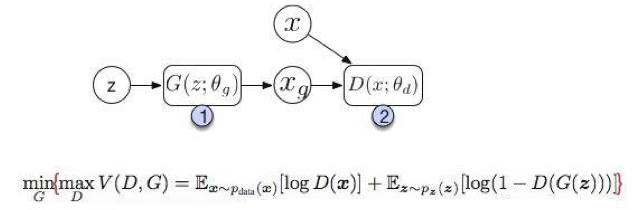
\includegraphics[totalheight=1.8in]{fig/standard_gan.png}
\caption{ 标准GAN算法示意图 } \label{fig:gansamples}
\end{figure}

最经典的GAN模型,由Ian Goodfellow提出,先从一个简单的分布中
采样一个噪声信号,然后经过生成函数后映射到我们想去拟合的数据分布
$x_g$。生成的数据和真实数据都会输入到一个识别网络D,识别网络
通过判别输出一个标量,表示数据来自真实数据的概率。在实现上,
要求G和D都是可微分函数,可以用多层神经网络来实现;后半部分是
模型训练中的目标函数。从公式上看,类似于CrossEntropy,注意到
D是P(Xdata)的近似。对于D来说,要尽量使公式最大化(识别能力强), 
而对于G又想使其最小。整个训练过程是一个迭代过程,但是在迭代中,
对D的优化又是内循环。生成模型可以发挥价值的场所: 
\begin{description}
	\item 特征表示
	\item 强化学习中的探索
	\item 逆强化学习
	\item 迁移学习
\end{description}



\begin{thebibliography}{99}
\addcontentsline{toc}{chapter}{\protect\numberline{}{\hspace{-1.5em}参考文献}}
\markboth{参考文献}{参考文献}
\bibitem{1} Gan导读,http://weibo.com/ttarticle/p/show?id=2309404060390806926698
\bibitem{2} John Glover, Modeling documents with generative adversarial networks, workshop on adversarial training, NIPS 2016, Barcelona, Spain

\end{thebibliography}

 
